\documentclass[a4paper 12pt]{article}

\usepackage[utf8]{inputenc}
\usepackage[T1]{fontenc}
\usepackage{mathptmx}
\usepackage{textcomp}
\usepackage[UKenglish]{babel}
\usepackage{xcolor}
\definecolor{codegreen}{rgb}{0,0.6,0}
\definecolor{codepurple}{rgb}{0.58,0,0.82}
\usepackage{listings}
\lstdefinestyle{code}{
	commentstyle=\color{codegreen},
	keywordstyle=\color{magenta},
	stringstyle=\color{codepurple},
	showspaces=false,
	showstringspaces=false,
	breaklines=true
}
\lstset{style=code}
\usepackage{amsmath, amssymb}
\usepackage{float}
\usepackage[hidelinks]{hyperref}
\hypersetup{
	colorlinks=false
}
\usepackage[style=ieee]{biblatex}
\bibliography{sources/biblio}
\renewcommand{\baselinestretch}{1.5}

\setlength{\parindent}{0pt}
\setlength{\parskip}{1em}

% figure support
\usepackage{import}
\usepackage{xifthen}
\pdfminorversion=7
\usepackage{pdfpages}
\usepackage{transparent}
\newcommand{\incfig}[1]{%
	\def\svgwidth{\columnwidth}
	\import{./figures/}{#1.pdf_tex}
}

\pdfsuppresswarningpagegroup=1

\begin{document}
\hypersetup{pageanchor=false}
\begin{titlepage}
  \begin{center}

    \textsc{\LARGE Dublin City University}\\[1cm]
    \textsc{\Large Electronic and Computer Engineering}\\[0.5cm]

    {\LARGE \bfseries EE514 Assignment\\[0.4cm]}
    {\Large \bfseries Fake News Detection\\[0.4cm]}

    \begin{figure}[H]
	
\includegraphics{images/Dcu-logo.png}
	\centering
    \end{figure}

    \vskip 2cm
    \emph{Author}\\[0.1cm]
    \noindent\makebox[\textwidth]{%
      \begin{tabular}{ll}%
        Michael Lenehan & michael.lenehan4@mail.dcu.ie \\
	Student Number: & 15410402 \\
    \end{tabular}}\\[0.1cm]

    \vfill

    % Bottom of the page
    % Probably replaced with date of deadline
    {\large{15/12/2019}}

  \end{center}
\end{titlepage}

\hypersetup{pageanchor=true}
\pagenumbering{alph}
\thispagestyle{plain}
\begingroup
\renewcommand{\cleardoublepage}{}
\renewcommand{\clearpage}{}

\LARGE{Declaration}

\endgroup

\vskip 1cm

I declare that this material, which I now submit for assessment, is entirely my
own work and has not been taken from the work of others, save and to the extent
that such work has been cited and acknowledged within the text of my work. I
understand that plagiarism, collusion, and copying are grave and serious
offences in the university and accept the penalties that would be imposed should
I engage in plagiarism, collusion or copying. I have read and understood the
Assignment Regulations set out in the module documentation. I have identified
and included the source of all facts, ideas, opinions, and viewpoints of others
in the assignment references. Direct quotations from books, journal articles,
internet sources, module text, or any other source whatsoever are acknowledged
and the source cited are identified in the assignment references. This
assignment, or any part of it, has not been previously submitted by me or any
other person for assessment on this or any other course of study.

I have read and understood the DCU Academic Integrity and Plagiarism at
\url{https://www4.dcu.ie/sites/default/files/policy/1%20-%20integrity_and_plagiarism\_ovpaa_v3.pdf}
and IEEE referencing guidelines found at
\url{https://loop.dcu.ie/mod/url/view.php?id=448779}.

\vskip 1cm
Signed: \underline{\ \ \ \ \ \ \ \ \ \ \ \ \ \ \ \ \ \ \ \ \ \ \ \ \ \ \ \ \ \ \
\ \ \ \ \ \ } \hspace{20mm}Date: \underline{15/12/2019}

\hspace*{0mm}\phantom{Signed:}Michael Lenehan

\pagebreak

\pagenumbering{arabic}
\tableofcontents
\clearpage
\section{Introduction}
With the explosion of information which has come with the prevalence of social
media, there has also come an explosion of misinformation. Machine Learning
techniques allow the opportunity to automatically determine whether the
information being served up is genuine, or satirical, or in simpler terms
``real'', or ``fake'' news.

\par With social media being one of the largest sources of shared misinformation, the
ability to flag suspect articles could lead to a large decrease in the amount of
misinformation in circulation. However, the classification of these articles
would need to be robust enough to avoid misclassifying, and mislabelling,
articles as ``fake'' or malicious.

\par Using a recently assembled dataset of satirical and non-satirical
headlines, a model can be trained in order to satisfy these requirements. This
assignment aims to investigate the implementation of such a model, and to
examine the accuracy which can be achieved.

\section{Preprocessing}
In the preprocessing stage, the dataset must first be loaded into the program, the
required data parsed from the dataset, and any inconsistencies within the
dataset must be accounted for. Iconsistencies can include missing data, or any
redundant or unnecessary data.

\par The provided ``fake-news'' dataset is stored in the ``JSON'' format. This
hierarchical data type makes parsing relatively simple. The ``loadData.py''
file contains two methods, one for loading the data into a pandas DataFrame object,
and one for defining the target values and the features within the dataset.

\begin{lstlisting}[language=Python, caption={``loadJson'' function},
label={lst:loadJson}]
def loadJson(jsonFile, printMsgs=False):
	jsonInput = pd.read_json(jsonFile, lines=True)
	if(printMsgs == True):
		print(jsonInput.head())
		print("Shape:", jsonInput.shape)
		print("\nFeatures:", jsonInput.columns)
	return jsonInput
\end{lstlisting}

The function shown in Listing \ref{lst:loadJson} utilises the pandas python
library, and it's provided ``read\_json'' function. This function loads a json
file, with the given file path, to a pandas DataFrame object. As the provided
dataset contains each json object on a new line, the ``lines'' parameter of the
``read\_json'' function must be set to ``True'', telling the function to treat
each newline as a new json object.

\begin{lstlisting}[language=Python, caption={``splitFeaturesAndTargets''
function}, label={lst:splitFAndT}]
def splitFeaturesAndTargets(data, printMsgs=False):
	x = data[data.columns[1:]]
	y = data[data.columns[0]]
    	if(printMsgs == True):
		print("Feature Matrix:", x.head())
		print("\nResponse Vector", y.head())
	return x, y
\end{lstlisting}

The function shown in Listing \ref{lst:splitFAndT} performs the split of the
features from the dataset. The features chosen are the ``headlines'', and the
``article links''. The targets are chosen as the ``is\_sarcastic'' value, which is
the ground truth, i.e. indicates whether the headline is deemed to be sarcastic,
and therefore fall into the category of ``fake news''

\subsection{Train and Test Split}

In order to accurately train and test a classification model, the dataset must
be divided into a training set, and a test set. This removes the possibility
that the model will ``memorize'' the entire dataset, giving a 100\% accuracy.
While performing this split, an unbiased training and test set must be created.
For example, training a model off entirely off ``sarcastic'' items would not
provide good accuracy during the testing phase.

\begin{lstlisting}[language=Python, caption={sklearn ``train\_test\_split''
function},
label={lst:ttsplit}]
X_train, X_test, y_train, y_test = train_test_split(
x, y , shuffle=True, test_size=0.25, random_state=1)
\end{lstlisting}

The scikit-learn python library contains a ``train\_test\_split'' function,
which, as shown in Listing \ref{lst:ttsplit}, can be used to split the feature
and target sets in the proportions given by the ``test\_size'' parameter. The
``shuffle'' parameter allows for the shuffling of the data, which will allow for
less biased split. The ``random\_state'' parameter sets the seed used by the
random number generator, allowing for repeatability within the
testing\cite{sk_ttsplit}.

The function call in Listing \ref{lst:ttsplit} creates a train test split of
75\% to 25\%, which is shuffled to remove bias, with a random state of 1 for
repeatability between tests.

\begin{lstlisting}[language=Python, caption={``countRealFake'' function},
label={lst:realFake}]
def countRealFake(targetTrainSet, targetTestSet):
    print("Real Headlines in Training Set: %s" % sum(targetTrainSet == 0))
    print("Fake Headlines in Training Set: %s" % sum(targetTrainSet == 1))
    print("Real Headlines in Test Set: %s" % sum(targetTestSet == 0))
    print("Fake Headlines in Test Set: %s" % sum(targetTestSet == 1))
\end{lstlisting}

In order to count the number of real and fake headlines within each set, the
``countRealFake'' function is used. This function takes two datasets, namely the
target training set, and the target test set, and prints the total number of
fake and real headlines in each, represented by a ``1'' or a ``0'' respectively.

\begin{lstlisting}[language=Python, caption={``exportTestTrain'' function},
label={lst:exporttt}]
def exportTestTrain(X_train, X_test, y_train, y_test, printMsgs=False):
	Export = X_train.to_json(r'./XTrain.json', orient='records')
	Export = X_test.to_json(r'./XTest.json', orient='records')
	Export = y_train.to_json(r'./YTrain.json', orient='records')
	Export = y_test.to_json(r'./YTest.json', orient='records')
	if(printMsgs == True):
		print("Training Features output to XTrain.json")
		print("Test Features output to XTest.json")
		print("Training Targets output to YTrain.json")
		print("Test Targets output to YTest.json")
\end{lstlisting}

In order to export the feature and target training and test sets, the
``exportTestTrain'' function is used. As shown in Listing \ref{lst:exporttt},
this function uses the pandas library ``to\_json'' function to output the json
object to a file. The ``orient'' parameter is set to ``records'' in order to
make the file more human readable.

\subsection{Feature Extraction}

For the purposes of feature extraction, a ``Bag of Words'' tokenizer is utilised
to count the occurrences of words within the headlines. The sklearn
``CountVectorizer'' function provides this functionality\cite{skcntVect}. There are a number of
tunable parameters with this function, however, the main concern for this
assignment is the inclusion or removal of ``stop words''. The headlines, and the
words of which they comprise are the features within this dataset.

\par TFIDF stands for Term-Frequency-Inverse Document Frequency. Term Frequency
is given in terms of each headline, i.e. how frequent a term is within the
headline, whereas inverse document frequency is the number of occurrences of the
word acrross all documents. Tf-Idf can be implemented in python using the
sklearn ``TfidfTransformer'' method, which can be configured to utilise, or
ignore, idf. A comparison of the inclusion or exclusion of idf is contained in
the Model Selection section.

\section{Exploratory Data Analysis}
By analysing the ``XTrain.json'' feature training set, some important
information can be found. For example, the file contains both the article
headline, and the article link. Training utilising the article link will give
100\% accuracy, as all fake news headlines are sourced from the satirical news
website ``The Onion'', while all real news headlines are sourced from the
``Huffington Post''. As such, models should only be fit using the article
headlines.

\begin{lstlisting}[language=Python, caption={``countTopWords'' Function},
label={lst:cntTopWords}]
def countTopWords(featureTrainCounts, count_vect, n):
    sum_words = featureTrainCounts.sum(axis=0)
    words_freq = [(word, sum_words[0, idx])
                  for word, idx in count_vect.vocabulary_.items()]
    words_freq = sorted(words_freq, key=lambda x: x[1], reverse=True)
    return words_freq
\end{lstlisting}

In order to count the most frequently occurring words in each feature, the
``countTopWords'' function is used. This function, as in Listing
\ref{lst:cntTopWords}, takes the matrix output of the ``CountVectorizer''
function, adds the occurrences of each word, and sorts the values into a list of
tuples of word-frequency pairs\cite{boujon_2019}. This list can then be returned
to the calling function.

In order to plot the most frequently occurring words within the training set,
the ``plotBagOfWords'' function is used. This function , as shown in Listing
\ref{lst:plotBOW}, takes a plot title, the
output from the ``countTopWords'' function, and the number of terms, and plots
them in a bar plot of words against frequency. This bar plot is plotted
horizontally for clearer readability.

\begin{lstlisting}[language=Python, caption={``plotBagOfWords'' Function},
label={lst:plotBOW}]
def plotBagOfWords(plotTitle, data, n):
    sns.set(style="darkgrid")
    x = []
    y = []
    for N in range(n):
        x += [data[N][0]]
        y += [data[N][1]]
        print(x)
        print(y)
    ax = sns.barplot(x=y, y=x, color="blue")
    ax.set(xlabel='Frequency', ylabel='Word', title=plotTitle)
    plt.show()
\end{lstlisting}

To test the difference in allowing or removing stop words - presumed
``uninformative'' words\cite{} - the ``bagOfWords'', ``countTopWords'', and
``plotBagOfWords'' functions must be called with the ``stopWords'' parameter set
to ``True'' and ``False''. The following plots show the differences when stop
words are and aren't included.

\begin{figure}[H]
	\centering
	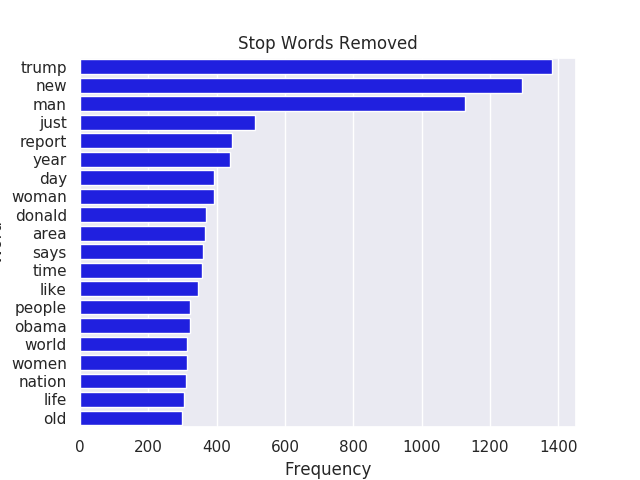
\includegraphics[width=0.8\textwidth]{images/stopWordsRemoved}
	\caption{Most Frequent Terms - Stop Words Removed}
	\label{fig:plotNoStops}
\end{figure}

\begin{figure}[H]
	\centering
	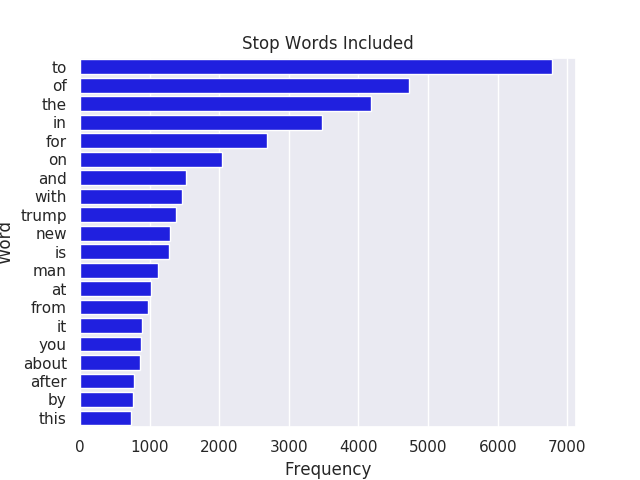
\includegraphics[width=0.8\textwidth]{images/stopWordsIncluded}
	\caption{Most Frequent Terms - Stop Words Included}
	\label{fig:plotStops}
\end{figure}

In order to verify these results, the ``yellowbrick'' library was used to
vizualize the data\cite{tfdYB}. The results from this verification can be seen in Figures
\ref{fig:plotNoStopsYB} and \ref{fig:plotStopsYB}.

\begin{figure}[H]
	\centering
	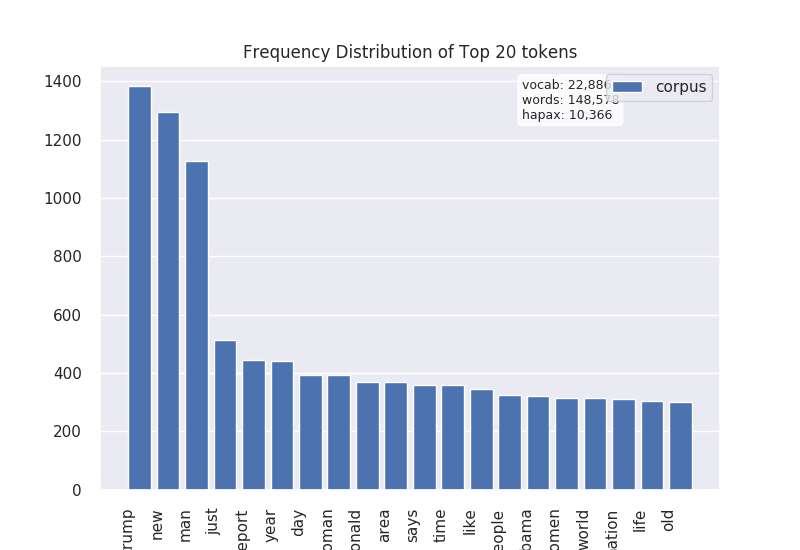
\includegraphics[width=0.8\textwidth]{images/SWRemovedYB}
	\caption{Most Frequent Terms - Stop Words Removed - Yellowbrick}
	\label{fig:plotNoStopsYB}
\end{figure}

\begin{figure}[H]
	\centering
	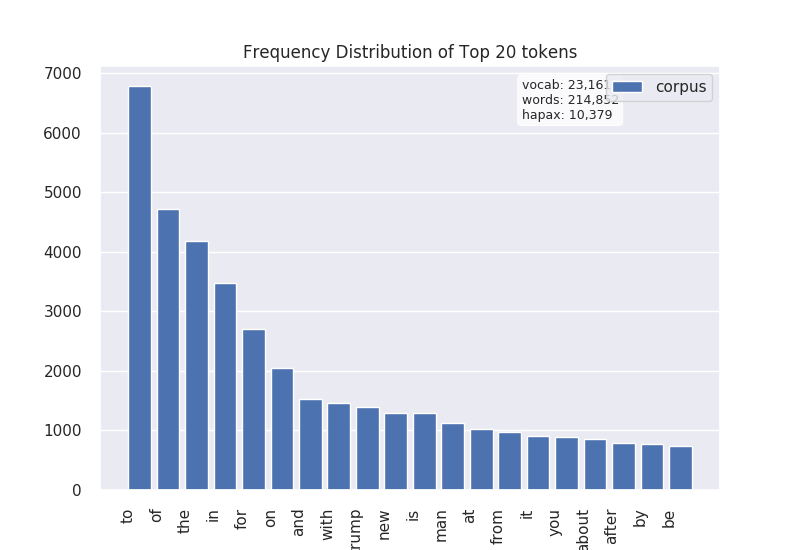
\includegraphics[width=0.8\textwidth]{images/SWIncludedYB}
	\caption{Most Frequent Terms - Stop Words Included - Yellowbrick}
	\label{fig:plotStopsYB}
\end{figure}

As seen in Figure \ref{fig:plotNoStops}, the most frequent word within the
training set, with stop words removed, is ``Trump''. This gives some context to
the nature of the content within the dataset. However, in Figure
\ref{fig:plotStops}, the most frequent word within the training set without
removing stop words is ``to''. This word gives no contextual information, and as
such, shows the benefits of removing stop words within the Bag of Words model.

\begin{lstlisting}[language=Python, caption={``countHeadlineLength'' Function},
label={lst:cntLength}]
def countHeadlineLength(features, target):
    fakeLen = np.array([])
    realLen = np.array([])
    for index, value in target.items():
        # print("Index: {}, Value: {}".format(index, value))
        if(value == 1):
            fakeLen = np.append(fakeLen, len(features.headline.loc[index]))
        else:
            realLen = np.append(realLen, len(features.headline.loc[index]))
        # print(features.headline.loc[index])
    print(np.mean(fakeLen))
    print(np.mean(realLen))
    plotHeadlineLength(fakeLen, realLen)
\end{lstlisting}

\par In addition to the frequency of the words, the length of the headlines can
be assessed. The ``countHeadlineLength'' function, as shown in Listing
\ref{lst:cntLength}, takes the feature and target datasets as inputs, iterates
over the target set, and creates two numpy arrays, one containing the length of
the ``real'' article headlines, and one with the ``fake'' articel headlines. The
mean value of these arrays can then be taken. In order to visualize this
information, two boxplots are drawn, using the seaborn library ``boxplot''
function. The ``plotHeadlineLength'' function takes in the real and fake
headline length arrays are passed in to the function, which converts each to a
pandas DataFrame object in order to plot them.

\begin{lstlisting}[language=Python, caption={``plotHeadlineLength'' Function},
label={lst:plotLength}]
def plotHeadlineLength(fake, real):
    dataFake = pd.DataFrame(fake)
    dataReal = pd.DataFrame(real)
    sns.set(style='darkgrid')
    ax = sns.boxplot(data=dataFake, orient="h")
    ax.set(xlabel='Headline Length', ylabel='', title="Fake Headline Length")
    plt.savefig('fakeHeadlineLength.png')
    plt.show()
    bx = sns.boxplot(data=dataReal, orient="h")
    bx.set(xlabel='Headline Length', ylabel='', title="Real Headline Length")
    plt.savefig('realHeadlineLength.png')
    plt.show()
\end{lstlisting}

The resulting boxplots from Listing \ref{lst:plotLength} for the fake and real
headlines are shown below in Figures \ref{fig:fakeLength}, and
\ref{fig:realLength} respectively.

\begin{figure}[H]
	\centering
	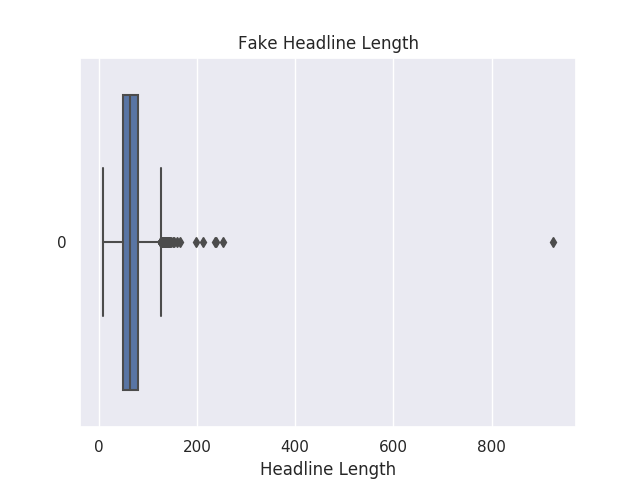
\includegraphics[width=0.8\textwidth]{images/fakeHeadlineLength}
	\caption{Lengths of the ``Fake'' Headlines}
	\label{fig:fakeLength}
\end{figure}

The mean length of a fake headline is approximately 65.48 characters. There is a
maximum length of 926 characters, and a minumum length of 8 characters.

\begin{figure}[H]
	\centering
	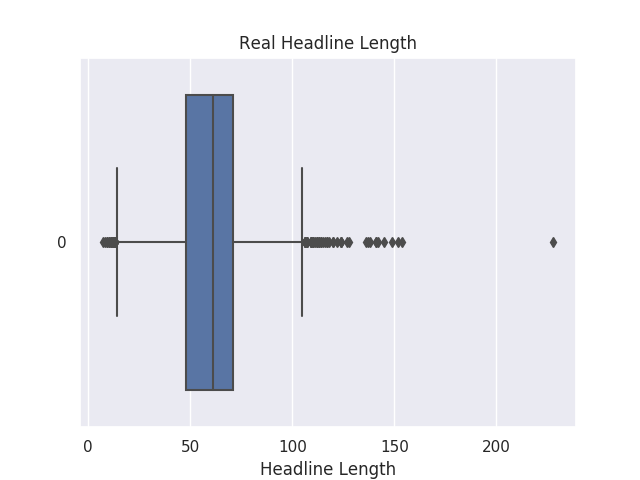
\includegraphics[width=0.8\textwidth]{images/realHeadlineLength}
	\caption{Lengths of the ``Real'' Headlines}
	\label{fig:realLength}
\end{figure}

The mean length of a real headline is approximately 59.46 characters. There is a
maximum length of 228 characters, and a minimum length of 7 characters.

\par From the above analysis it can be seen that the length of headlines for
fake headlines are, on average, longer, with a greater value outlier. As such,
the length of real headlines are shorter, with smaller outlier values.

\section{Supervised Classification}
Supervised Classigication involves training a supervised model based on the
aforementioned features, using a validation set. Due to an error which was
occurring - values within the target set changing to ``NaN'' - the chosen
cross validation method of ``Leave One Out'' cross validation could not be
correctly implemented, however, the tested implementation is commented within
the code. As such, only the held-out test set could be used for the purpose of
validation.

\par The ``Pipeline'' function is used to quickly create a model, allowing for
the vectorizer, tfidf function, and classifier to be applied to the training
sets for the features and targets. The models are saved using the ``pickle''
library's ``dump'' function. Each optimised model is saved after fitting.

\section{Model Selection}
For the purposes of classification within this assignment, the naive Bayes, and
Support Vector Machine (SVM) with Stochastic Gradient Descent are utilised. The
sklearn function ``MultinomialNB'' provides the naive Bayes classifier for the
model\cite{skBayes}. Using this classifier, a test accuracy of approximately
83\% was achieved.

\par For the SGD classifier, the sklearn function ``SGDClassifier'' was used.
This function takes the loss function, in this case a linear SVM is used by
implementing the ``hinge'' loss function. The standard linear SVM ``l2'' penalty
is also used. This classifier gives a test accurracy of approximately 79\%.

By utilising the sklearn ``GridSearchCV'' function, a number of parameters can
be tested for each model.

For the Naive Bayed model, the defined parameters were as follows:

\begin{lstlisting}[language=Python, caption={Bayes Model Parameters},
label={lst:bayesParam}]
parameters = {
    'vect__stop_words': (None, "english"),
    'vect__ngram_range': [(1, 1), (1, 2)],
    'tfidf__use_idf': (True, False),
    'clf__alpha': (1e-5, 1),
    'clf__fit_prior': (True, False),
}
\end{lstlisting}

By utilising this function, a ``best case'' model can be created. The model
described by the parameters above has a best score of approximately 85\%. The
parameters required for this performance were as follows:

\begin{itemize}
	\item Classifier:
	\begin{itemize}
		\item Alpha = 1
		\item Fit Prior = False
	\end{itemize}
	\item Feature Selection:
	\begin{itemize}
		\item Tf-Idf:
		\begin{itemize}
			\item Use Idf = False
			\item ngram Range = (1,2)
		\end{itemize}
		\item Count Vectorizer:
		\begin{itemize}
			\item Stop Words = None
		\end{itemize}
	\end{itemize}
\end{itemize}

For the SGD model, the defined parameters were as
follows:

\begin{lstlisting}[language=Python, caption={SGD Model Parameters},
label={lst:sgdParam}]
parameters = {
    'vect__stop_words': (None, "english"),
    'vect__ngram_range': [(1, 1), (1, 2)],
    'tfidf__use_idf': (True, False),
    'clf__alpha': (1e-2, 1e-3),
    'clf__loss': ('hinge', 'log'),
    'clf__max_iter': (1, 2, 3, 4, 5),
    'clf__shuffle': (True, False),
}
\end{lstlisting}

By utilising this function, a ``best case'' model can be created. The model
described by the parameters above has a best score of approximately 81\%. The
parameters required for this performance were as follows:

\begin{itemize}
	\item Classifier:
	\begin{itemize}
		\item Alpha = 0.001
		\item Loss Function = Log
		\item Max Iterations = 1
		\item Shuffle = True
	\end{itemize}
	\item Feature Selection:
	\begin{itemize}
		\item Tf-Idf
		\begin{itemize}
			\item Use Idf = True
			\item ngram Range = (1,1)
		\end{itemize}
		\item Count Vectorizer
		\begin{itemize}
			\item Stop Words = None
		\end{itemize}
	\end{itemize}
\end{itemize}

\section{Model Evaluation}
In order to evaluate both models, the sklearn ``metrics'' library was used, in
particular, the ``classification\_report'', and ``confusion\_matrix'' functions.
The classification reports, shown in Figures \ref{fig:bayesReport} and
\ref{fig:sgdReport} show the Precision, Recall, and F1 Score of each of the
``best case'' models, as described in the preceding section.

\begin{figure}[H]
	\centering
	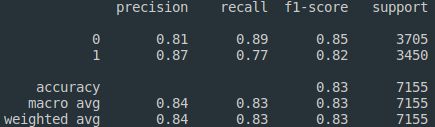
\includegraphics[width=0.8\textwidth]{images/bayesMetricReport}
	\caption{Metrics Report for the Bayes Model}
	\label{fig:bayesReport}
\end{figure}

Precision is defined as the models ability to minimize false positives, i.e.
only label positive data as positive data\cite{skMetric}. As can be seen in the
metrics report for the Bayes model, the precision for ``fake'' articles is
87\%, while the precision for the ``real'' articles is 81\%. Comparing this to
the SGD Model, it can be seen that the precision for ``real'' articles was much
higher in the case of the SGD Model, however there is a much lower value for
precision for the ``fake'' articles.

Recall is defined as the models ability to find all positive
matches\cite{skMetric}. Within the Bayes model, the recall for the ``real''
articles is 89\%, while for ``fake'' articles there is a value of 77\%.
Comparing with the SGD Model, there is a value of only 69\% for the ``real''
articles, with a value of 90\%  for the ``fake'' articles.

Finally, the F score is a weighted average of the precision and recall values.
The Bayes has an F score of 85\% for the ``real'' articles, with a value of 82\%
for the ``fake articles''. The SGD Model has a value of 77\% for the ``real''
articles, with a value of 80\% for the fake articles.

\begin{figure}[H]
	\centering
	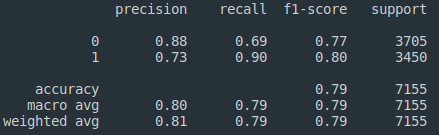
\includegraphics[width=0.8\textwidth]{images/sgdMetricReport}
	\caption{Metrics Report for the SGD Model}
	\label{fig:sgdReport}
\end{figure}

From these classification reports, it is clear that the Bayes classifier is
superior for this classification task. It has a better average precision and
recall for both article types. While the SGD classifier had better precision for
``real'' articles, and better recall for ``fake'' articles than the Bayes
classifier, the overall performance results in a lower oeverall accurracy.

The confusion matrices, as shown below in figures \ref{fig:bayesConf} and
\ref{fig:sgdConf} confirm the evaluation above. The number of false positives
within the Bayes classifier is much lower than that of the SGD Classifier,
however the number of false negatives within the SGD classifier is much lower
than that of the Bayes classifier. Again, the difference leaves a greater
accuracy for the Bayes classifier, making it a more optimal solution for this
assignment.

\begin{figure}[H]
	\centering
	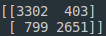
\includegraphics[width=0.8\textwidth]{images/bayesConfMatrix}
	\caption{Confusion Matrix for the Bayes Model}
	\label{fig:bayesConf}
\end{figure}


\begin{figure}[H]
	\centering
	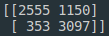
\includegraphics[width=0.8\textwidth]{images/sgdConfMatrix}
	\caption{Confusion Matrix for the SGD Model}
	\label{fig:sgdConf}
\end{figure}

\section{Conclusion}
While there were a number of requirements not completely satisfied within this
assignment, there are a number of conclusions which can be drawn.

\par In general the Multinomial Naive Bayes Classifier model achieved much
greater accuracy than the Stochastic Gradient Descent model. With an approximate
difference of 4\% in the accuracies achieved. The difference achieved could have
been much greater, had a correct implementation of Leave One Out Cross
Validation been utilised.

\par The evaluation of the models showed the differences in precision and
recall for the ``best case'' models, and the confusion matrices provided show
the number of false positives and false negatives for each model.

\par Overall, the Naive Bayes Classifier model achieved better overall accuracy
due to it's higher recall for ``real'' articles, and higher precision for
``fake'' articles. These attributes allowed for the much lower false positives,
and relatively low false negatives.

\clearpage
\section{Appendix}

The following is the main code body for the assignment. All other code can be
found in the code submission, or on github at \url{https://github.com/mLenehan1/EE514-DataAnalysis\\AndMachineLearning}

\par In order to execute the code, place all required python files in the working
directory, along with the dataset, and run ``python3 assignmentMain.py'' via the command line.
\lstinputlisting[language=Python]{sections/appendix/assignmentMain.py}
\clearpage
\printbibliography
\end{document}
